%!TEX root = "../../../DA_GUI.tex"

%	--------------------------------------------------------
% 	Debugger: Darstellung der Variablen
%	--------------------------------------------------------

%	--------------------------------------------------------
% 	Einführung + Erklärung Variablendarstellung
%	--------------------------------------------------------
\section{Darstellungsform der Variablen}

Zur Darstellung der Variablen während des Programmablaufes wurden zwei Konzepte verfolgt:
\begin{enumerate}
\item Die Anzeige des Call Stacks als Liste mit separaten Tabellen für die globalen und lokalen Variablen, Abbildung \ref{fig:deb-var-m1}.
\item Die Anordnung aller Variablen in einem Baum, wobei lokale Variablen Funktionen untergeordnet sind, Abbildung \ref{fig:deb-var-m2}.
\end{enumerate}

\begin{figure}[h!]
\centering
	\begin{minipage}{0.50\textwidth}
		\centering
		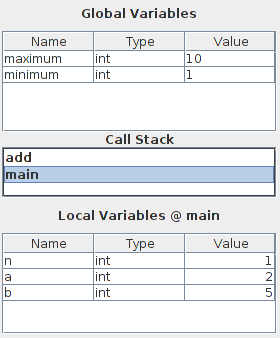
\includegraphics[width=1.0\textwidth]{./media/images/gui/var/callstack.png}
		\caption{Darstellung der Variablen als Liste}\label{fig:deb-var-m1}
	\end{minipage}\hfill
	\begin{minipage}{0.45\textwidth}
		\centering
		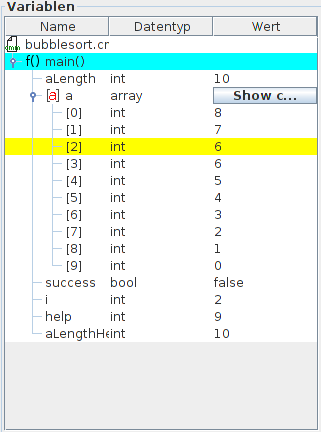
\includegraphics[width=1.0\textwidth]{./media/images/gui/var/treetable2.png}
		\caption{Darstellung der Variablen als Baum}\label{fig:deb-var-m2}
	\end{minipage}
\end{figure}

In den ersten Versionen der Benutzeroberfläche wurden die Variablen wie in Punkt 1 beschrieben dargestellt. Bereits während unseres Praktikums am Institut für Systemsoftware der JKU wurde die zweite Form der Variablendarstellung theoretisch entworfen. Die erste grundlegende Implementierung erfolgete noch während der Sommerferien.

%TODO ref versionsgeschichte
In der ersten numerierten Version (Alpha 1.0) waren noch beide Darstellungsformen vorhanden und konnten vom Benutzer ausgewählt und gewechselt werden. Allerdings waren diese beiden Darstellungsformen sehr unterschiedlich implementiert, was Anfangs dazu führte, dass die Darstellung der Variablen als Baum nicht mehr als ein zusätzliches Feature ohne den vollen Funktionsumfang der Variablendarstellung als Call Stack war.

Für die Version Alpha 1.1 sollte ursprünglich das Variablendarstellungssystem so verändert werden, dass beide Anzeigemodi über ein gemeinsames Interface angesprochen werden können. Nach ausführlicher Besprechung und Evaluierung der unterschiedlichen Variablendarstellungen haben wir aber beschlossen, die Variablen nur als Baum darzustellen. Dadurch haben sich folgende Vorteile ergeben:
\begin{enumerate}
\item Die Implementierung einer neuen Funktion in der Variablenanzeige muss nur noch einmal erfolgen und nicht für jeden Anzeigemodus extra vorgenommen werden.
\item Daraus resultiert auch ein durchdachteres und einfacheres Bedienungskonzept der Benutezroberfläche, da dieses nur an eine Variablendarstellung angepasst werden muss.
\item Davon profitiert zuletzt der Benutzer, der eine komplette und sauber implementierte Anzeige und Erklärung der Variablen während des Programmablaufes vorfindet.
\end{enumerate}

%	--------------------------------------------------------
% 	Darstellung in getrennten Tabellen
%	--------------------------------------------------------
\section{Darstellung der Variablen in getrennten Tabellen}

Diese Form der Variablendarstellung wurde erstmals im Dokument Ausführungsumgebung für C-- von Herrn Professor Blachek beschrieben und nach dieser Vorlage implementiert\footnote{Ausführungsumgebung für C--, Günther Blaschek, V1.0, 2014-06-18}. Ein Vorteil dieser Darstellungsform war die Übersichtlichkeit und Einfachheit besonders beim Debuggen von einfachen Programmen. Leider verlor das Konzept an Übersichtlichkeit, wenn fortgeschrittene Programme mit komplexen Strukturen abgearbeitet wurden. Eine Tabelle konnte jeweils nur eine Ebene der Variablen, also beispielsweise den Inhalt einer Struktur oder die lokalen Variablen einer Funktion anzeigen.

%	--------------------------------------------------------
% 	Darstellung als Baum
%	--------------------------------------------------------
\section{Darstellung der Variablen als Baum}

\subsection{Darstellungsschema}

Die Darstellung der Variablen in Form einer Baumstruktur hat den Vorteil, dass alle Variablen in einem Feld untergebracht sind und die Gültigkeitsbereiche der Variablen sofort ersichtlich sind.

Die TreeTable besitzt drei Spalten: In der ersten befindet sich der Baum mit den Namen der Variablen. in der zweiten Spalte wird der Datentyp der Variable und in der dritten ihr Wert gezeigt.

Alle Elemente befinden sich in einem Ordner, der den Namen der Datei trägt. Dadurch wird symbolisiert, dass die Variablen ein Teil des Programms sind. Dem Programm selbst untergeordnet sind globale Variablen und Funktionen. Lokale Variablen sind Funktionen untergeordnet, Variablen in Strukturen sind der Struktur untergeordnet.
Zusätzlich werden folgende Elemente in der Tabelle farbig markiert:
\begin{itemize}
\item Funktionen sind hellblau hinterlegt. Sie sollen dadurch optisch von Datenstrukturen und Variablen unterscheidbar sein.
\item Die Variablen, die zuletzt geändert wurden, sind gelb hinterlegt. Grundsätzlich kann pro Schritt des Debuggers nur eine Variable geändert werden. Werden aber einige Schritte übersprungen, zum Beispiel mit dem Schlüsselwort \glqq{}library\grqq{}, so werden mehrere Variablen in einem Debuggerschritt geändert.
% TODO refer to library
\item Variablen, die noch nicht initialisiert wurden, sind grau hinterlegt.
% TODO refer to undef variables
\end{itemize}

\begin{figure}[htp]
\centering
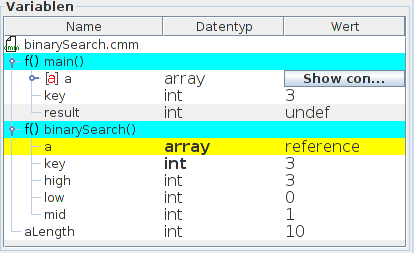
\includegraphics[width=0.5\textwidth]{/home/fabian/Dokumente/C--/CMM/doc/de/media/images/gui/debugger/gui-treetable.png}
\caption{Beispiel für farbige Hervorhebung von Variablen}
\label{fig:deb-tt-example}
\end{figure}

%    ---------------------------------------------------------------------
%        Grundlegende Komponenten
%    ---------------------------------------------------------------------

\subsection{Grundlegende Komponenten}
Die Variablen werden in einer Tabelle mit Baumstruktur, deshalb auch ,,TreeTable'' genannt, angezeigt. Die TreeTable ist eine Kombination aus einem JTree und einer JTable.
Im Folgenden werden diese Komponenten beschrieben und der Aufbau der TreeTable erläutert.

\subsubsection*{JTree - Baum}

\begin{wrapfigure}{r}{0.35\textwidth}
  	\begin{center}
    	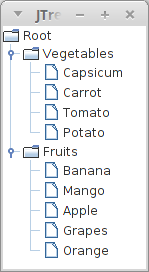
\includegraphics[width=0.3\textwidth]{./media/images/gui/debugger/JTree-Example.png}
  	\end{center}
  	\caption{Beispiel für einen einfachen Baum}
	\label{fig:deb-tt-example-jtree}
\end{wrapfigure}

Ein JTree\footnote{http://www.codejava.net/java-se/swing/jtree-basic-tutorial-and-examples} ist Swing-Element, das Daten hierarchisch untereinander darstellet. Die Daten sind allerdings nicht im JTree selbst gespeichert, sondern in externen Objekten. Ein JTree kann entweder mit einem Datenmodell oder mit dem Hauptknoten eines Baumes initialisiert werden\footnote{http://docs.oracle.com/javase/tutorial/uiswing/components/tree.html}. Da die Daten eines JTree einen Baum abbildet, kann durch diese Struktur traversiert werden. Solche Operationen\footnote{http://www.java-tutorial.ch/core-java-tutorial/expande-or-collapse-all-nodes-in-a-jtree} werden beispielsweise benötigt, um alle Knoten eines Baumes zu öffnen (expand) oder zu schließen (collapse).

Wird ein JTree direkt mit einem Baum initialisiert, müssen die Knoten das Interface TreeNode implementieren\footnote{http://docs.oracle.com/javase/7/docs/api/javax/swing/tree/TreeNode.html}. Für einfache Aufgaben können Standardklassen, wie etwa DefaultMutableTreeNode\footnote{https://docs.oracle.com/javase/7/docs/api/javax/swing/tree/DefaultMutableTreeNode.html} verwendet werden.
Mehr Möglichkeiten bietet aber die explizite Verwedung eines Datenmodells. Ein Datenmodell regelt die Interaktion des JTree mit seinem Datenbaum und stellt Methoden zum Einfügen, Löschen und Ändern von Knoten sowie zum Auslesen des Pfades eines Knotens zur Verfügung.
Der JTree in der TreeTable von C Compact verwendet ein eigenes Datenmodell, TreeTableDataModel. Der Baum besteht aus Objekten der Klasse DataNode. Da ein eigenes Datenmodell verwendet wird, muss DataNode das Interface TreeNode nicht implementieren.

\subsubsection*{JTable - Tabelle}
Tabellen können in Swing mit dem Komponenten JTable\footnote{http://docs.oracle.com/javase/tutorial/uiswing/components/table.html} dargestellt werden. Wie auch bei der Klasse JTree werden die Daten nicht im Objekt von JTable gespeichert. Im einfachsten Fall kann eine Tabelle durch ein zweidimensionales Array initialisiert werden\footnote{http://www.java2s.com/Tutorial/Java/0240\_\_Swing/CreatingaJTable.htm}. In der Regel wird aber ein Datenmodell wie etwa DefaultTableModel\footnote{http://docs.oracle.com/javase/8/docs/api/javax/swing/table/DefaultTableModel.html} verwendet. Ein für eine Tabelle verwendbares Datenmodell ist ein Objekt einer Klasse, die das Interface TableModel\footnote{http://docs.oracle.com/javase/8/docs/api/javax/swing/table/TableModel.html} implementiert.

\begin{figure}[h]
\centering
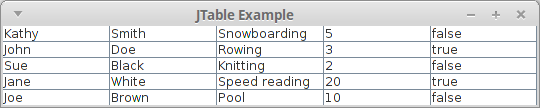
\includegraphics[width=0.5\textwidth]{./media/images/gui/debugger/JTable-Example.png}
\caption{Beispiel für eine einfache Tabelle}
\label{fig:deb-tt-example-jtable}
\end{figure}

%    ---------------------------------------------------------------------
%        Allgemeine Implementierung
%    ---------------------------------------------------------------------

\subsection{Allgemeine Implementierung}
Die grundlegende Implementierung erfolgte anhand eines Blogeintrages\footnote{http://www.hameister.org/JavaSwingTreeTable.html}, mittlerweile wurde der Code allerdings stark an die Anforderungen der Benutzeroberfläche angepasst und erweitert.

Da die TreeTable auch zum Auswählen der Questpackete verwendet wird, wurde ein Großteil allgemein implementiert, sodass die TreeTable auch für andere Anwendungen ohne Probleme weiterverwendet werden kann. Für jede Anwendung muss eine eigene Klasse als Knoten des Baumes der TreeTable erstellt werden. Optional ist die Erweiterung durch einen eigenen Renderer, der den Elementen der TreeTable unterschiedliche Symbole gibt.

Im folgenden Klassendiagramm wird der Aufbau der TreeTable dargestellt. Swing - Komponenten sind Dunkelblau, von Java vorgegebene Klassen und Interfaces sind Hellblau dargestellt. Die meisten Klassen sind selbst implementiert und daher mit weiß gekennzeichnet. Orange gefärbte Klassen müssen für die jeweilige Anwendung extra geschrieben bzw. angepasst werden.

Alle Klassen der TreeTable, die allgemein verwendet werden können, befinden sich im Packet \textbf{at.jku.ssw.cmm.gui.treetable}.

\begin{figure}
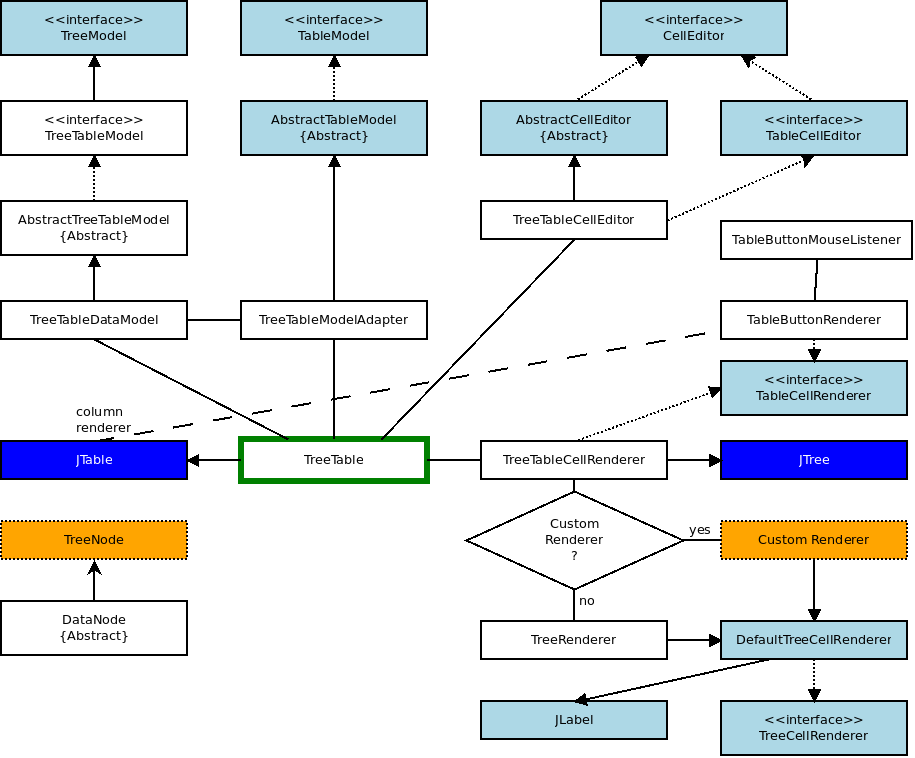
\includegraphics[width=\textwidth]{./media/images/gui/var/TreeTableClassesRaw.png}
\caption{Allgemeines Klassendiagramm der TreeTable}
\label{fig:deb-var-tt-class-raw}
\end{figure}

\subsubsection*{TreeTable.java}
Diese Klasse ist die Hauptklasse der TreeTable und, da sie von JTable erbt, eine Swing-Komponente. Hier laufen alle Teile der TreeTable, wie etwa Datenmodelle und Renderer, zusammen.

Im Konstruktor werden einige Einstellungen an der Tablelle geändert. Diese Einstellungen können auch über die TreeTable selbst geädert werden (da sie von JTable erbt), allerdings sollte das vertauschen der Tabellenspalten deaktiviert bleiben (da sonst Probleme mit den Renderen des Baumes auftreten können).
\begin{lstlisting}[language=JAVA]
public TreeTable( TreeTableDataModel<TreeNode> treeTableModel ){
    super();
    this.setTreeModel(treeTableModel);
        
    //Do not allow column reordering
    getTableHeader().setReorderingAllowed(false);
        
    //Do not show the table grid
    setShowGrid(false);
        
    //No spacing
	setIntercellSpacing(new Dimension(0, 0));
}
\end{lstlisting}

Die Klasse \textbf{TreeTable} enthält zwei Methoden, die für die Implementierung besonders wichtig sind:
\begin{lstlisting}[language=JAVA]
public void setTreeModel( TreeTableDataModel<TreeNode> treeTableModel );
public void updateTreeModel();
\end{lstlisting}

Beide Methoden aktualisieren die angezeigten Daten in der TreeTable. Die Methode \textbf{setTreeModel(...)} muss verwendet werden, wenn ein neues Datenmodell angezeigt werden soll oder wenn sich die Struktur des Baumes verändert hat. Nach einfachen Wertänderungen in einem oder mehreren Knoten kann die Methode \textbf{updateTreeModel()} aufgerufen werden.

\subsection*{DataNode}
Ein Datenknoten (DataNode) ist ein Knoten des in der TreeTable abgebildeten Baumes. In diesen Knoten sind alle nötigen Informationen zu den angezeigten Variablen - auch jene, die nicht im Baum selbst sondern in der Tabelle angezeigt werden - gespeichert. Ein Knoten speichert immer alle Informationen einer ganzen Zeile.

DataNode ist eine abstrakte Basisklasse, die alle Daten enthält, diezur Verwendung in der TreeTable notwending sind. Für die Anwendung muss eine eigene Node-Klasse implementiert werden, die von DataNode erbt.

\begin{lstlisting}[language=JAVA]
public abstract class DataNode {
	public abstract List<DataNode> getChildren();
	public abstract int getChildCount();
	public abstract Object getValueByColumn(int col);
	public abstract void addChild(DataNode n);
	@Override
	public abstract String toString();
	public void add(DataNode subNode) {
		// TODO Auto-generated method stub
		
	}
}
\end{lstlisting}

Eine Verknüpfung zu allen Kindknoten (bestenfalls als \textbf{List}) muss in der abgeleiteten Klasse erfolgen. Die \textbf{toString}-Methode muss überschrieben werden, da diese für den Baum verwendet wird. \textbf{toString} sollte also den Namen des Datenknoten übergeben. Die Implementierung der Methode \textbf{add} ist empfehlenswert (da der Baum irgendwie aufgebaut werden muss), aber nicht erforderlich.

\subsubsection*{TreeModel.java}
TreeModel ist ein Interface für alle Datenmodelle eines JTree.

\subsubsection*{TreeTableModel.java}
Dieses Interface erweitert das Interface TreeModel so, dass es mit einer TreeTable kompatibel wird. TreeTableModel definiert zusätzliche Methoden, die für das Datenmodell einer Tabelle benötigt werden, beispielsweise \textbf{getColumnName()}.

\subsubsection*{AbstractTreeTableModel.java}
Diese abstrakte Basisklasse implementiert einige konkrete Methoden für die Verwendung als Datenmodell eines JTree. In Objekten dieser Klasse werden der Hauptnoten (root) des Baumes gespeichert. Außerdem regelt AbstractTreeModel den Ablauf von Änderungsevents in der Datenstruktur des Baumes.

\subsubsection*{TreeTableDataModel.java}
TreeTableDataModel erbt von AbstractTreeTableModel und ist das komplette Tabellen-Datenmodell. Es sind einige Methoden implementiert, die im Datenmodell einer Tabelle benötigt werden. Außerdem wird in dieser Klasse das kontrete Aussehen der Tabelle festgelegt, indem die Tabellenspalten definiert werden.

Um die TreeTable zu initialisieren, muss ein Datenmodell von dieser Klasse erstellt werden. Dabei müssen der Hauptknoten des Datenbaumes (mit Knoten, die von \textbf{DataNode} erben) und Namen und Datentypen der Tabellenspalten angegeben werden.
%TODO ref rederer for special datatypes
\begin{lstlisting}[language=JAVA]
public class TreeTableDataModel<TreeNode extends DataNode> extends AbstractTreeTableModel<TreeNode> {

	public TreeTableDataModel(TreeNode rootNode, String[] columnNames, Class<?>[] columnTypes, int currFunc) {
		super(rootNode);
		...
    }
    ...
}
\end{lstlisting}

\subsubsection*{TableModel.java}
Dieses Interface bildet die Grundlage für alle Datenmodelle einer JTable\footnote{http://docs.oracle.com/javase/7/docs/api/javax/swing/table/TableModel.html}.

\subsubsection*{AbstractTableModel.java}
In dieser abstrakten Basisklasse sind bereits die meisten Methoden des Interface TreeModel implementiert\footnote{http://docs.oracle.com/javase/7/docs/api/javax/swing/table/AbstractTableModel.html}. Alle dazu noch benötigten Methoden werden in der Klasse \textbf{TreeTableModelAdapter} definiert.

\subsubsection*{TreeTableModelAdapter.java}
TreeTableModelAdapter bildet die Verbindung zwischen dem Datenmodell der Tabelle und dem des Baumes. Diese Klasse erbt von AbstractTreeTableModel und enthält eine Referenz auf TreeTableDataModel. Viele Methoden, wie etwa ,,getColumnName()'' oder ,,getValueAt()'' sind in TreeTableDataModel implementiert, da sich in dieser Klasse auch das eigentliche Datenmodell der TreeTable befindet, und werden in TreeTableModelAdapter übernommen. Beispielsweise greifen die folgenden Methoden auf die Implementierung in TreeTableDataModel zurück:
\begin{lstlisting}[language=JAVA]
public Object getValueAt(int row, int column) {
   return treeTableModel.getValueAt(nodeForRow(row), column);
}

public boolean isCellEditable(int row, int column) {
   return treeTableModel.isCellEditable(nodeForRow(row), column);
}
\end{lstlisting}

\subsubsection*{CellEditor.java}
Dieses Interface bildet die Grundlage für alle Klassen, die CellEditor einer JTable sind\footnote{https://docs.oracle.com/javase/7/docs/api/javax/swing/CellEditor.html}.
Ein CellEditor ist für die Dateneingabe in eine Tabelle verantwortlich\footnote{http://docs.oracle.com/javase/tutorial/uiswing/components/table.html\#editor}. Die einfachse Form eines CellEditors ist ein DefaultCellEditor\footnote{https://docs.oracle.com/javase/7/docs/api/javax/swing/DefaultCellEditor.html}. Dieser unterstützt die Eingabe von Daten in die Tabelle mithilfe eines Textfeldes, einer Checkbox oder einer Combobox.

\subsubsection*{AbstractCellEditor.java}
AbstractCellEditor ist eine abstrakte Basisklasse für alle Arten eines CellEditor in Swing\footnote{https://docs.oracle.com/javase/7/docs/api/javax/swing/AbstractCellEditor.html}. Einige grundlegende Methoden sind bereits implementiert.

\subsubsection*{TableCellEditor}
Dieses Interface\footnote{http://docs.oracle.com/javase/7/docs/api/javax/swing/table/TableCellEditor.html} definiert die Methode \textbf{getTableCellEditorComponent(...)}. Diese Methode sollte den Kompontenten der Tabelle bzw. der betroffenen Zelle zurückgeben, der verwendet wird, um den Inhalt zu modifizieren.

\subsubsection*{TreeTableCellEditor.java}
Daten in der TreeTable sollen vom Benutzer zwar nicht verändert werden können, wenn das Editieren der Tabelle mit der Methode \glqq{}setEditable()\grqq{} aber deaktiviert wird, werden auch Events (wie etwa Mausklicks) nicht mehr registriert. TreeTableCellEditor gibt also Events in der Tabelle bei Bedarf an den JTree weiter und verbietet Events in Zellen, die nur Text enthalten.
\begin{lstlisting}[language=JAVA]
public boolean isCellEditable(EventObject e) {
	if (e instanceof MouseEvent) {
     	MouseEvent me = (MouseEvent) e;
    	MouseEvent newME = new MouseEvent(tree, me.getID(), me.getWhen(), me.getModifiers(), me.getX() - table.getCellRect(0, 0, true).x, me.getY(), 2, me.isPopupTrigger());
    	tree.dispatchEvent(newME);
  	}
  	return false;
}
\end{lstlisting}

Außerdem wird die Methode \textbf{getTableCellEditorComponent(...)} implementiert, die je nach der betroffenen Spalte entweder die Tabelle selbst oder den Baum als zuständiges Swing-Element angibt.
\begin{lstlisting}[language=JAVA]
public Component getTableCellEditorComponent(JTable table, Object value, boolean isSelected, int r, int c) {
    if( c == 0 )
        return this.tree;
    else
        return this.table;
}
\end{lstlisting}

\subsubsection*{TableCellRenderer.java}
In diesem Interface sind alle Methoden definiert, die zum Rendern von Zellen einer JTable benötigt werden\footnote{https://docs.oracle.com/javase/7/docs/api/javax/swing/table/TableCellRenderer.html}.

%TODO TODO TODO missing: TableButtonMouseListener, (swing)
\subsubsection*{TableButtonRenderer.java}
Diese Klasse sorgt dafür, dass die Zellen der Tabelle die richtige Hintergrundfarbe erhalten und dass AWT- und Swing-Elemente in der Tabelle richtig dargestellt werden. Um Elemente der grafischen Benutzeroberfläche in einer Tabelle zu rendern, muss die Methode \textbf{getTableCellRendererComponent(...)} für die jeweilige Zelle das beinhaltete Element zurückgeben.
\begin{lstlisting}[language=JAVA]
public Component getTableCellRendererComponent(JTable table, Object value, boolean isSelected, boolean hasFocus, int row, int column) {
	Component c = (Component)defaultRenderer.getTableCellRendererComponent(table, value, isSelected, hasFocus, row, column);
	
	// AWT- oder Swing-Komponente verwenden
	if(value instanceof Component)
		return (Component)value;
	
	// Weitere Anpassungen
	else if( ... )
		...
	
	return c;
}
\end{lstlisting}

\subsubsection*{TreeTableButtonMouseListener.java}
Diese Klasse implementiert das Interface \textbf{MouseListener} und ist Event Listener der gesamten TreeTable. Dieser Listener muss allerdings manuell zur TreeTable hinzugefügt werden.
\begin{lstlisting}[language=JAVA]
treeTable.addMouseListener(new TableButtonMouseListener(main, treeTable));
\end{lstlisting}

Der Listener \textbf{TreeTableButtonMouseListener} sorgt dafür dass, falls ein Button in der Tabelle angeklickt wird, der entstandene Event an den Button weitergeleitet wird, sodass der Button seinen eigenen EventListener ausführen kann.
\begin{lstlisting}[language=JAVA]
public void mouseClicked(MouseEvent e) {
	// Leitet den Event an den angeklickten Button weiter
	forwardEventToButton(e, this.treeTable.getTable().rowAtPoint(e.getPoint()), this.treeTable.getTable().columnAtPoint(e.getPoint()));
}
\end{lstlisting}

\subsubsection*{TreeTableCellRenderer.java}
Diese Klasse erbt von JTree und wird verwendet, um einen Baum in die erste Spalte der Treetable, also die Spalte mit de Baum - zu rendern. Außerdem ist diese Klasse dafür verantwortlich, dass die Zeilen der Tabelle und des Baumes die selbe Höhe haben und dass die Zellen die richtige Farbe erhalten.
%TODO refer to table line colors

An den JTree selbst kann außerdem noch ein eigens erstellter Renderer übergeben werden, um beispielsweise eigene Symbole für jeden Knoten im Baum anzuzeigen. Dieser Renderer muss das Interface \textbf{DefaultTreeCellRenderer} implementieren. Ist ein solcher Renderer nicht vorhanden, wird die standardmäßig \textbf{TreeRenderer} verwendet.

\subsubsection*{JLabel.java}
Ein JLabel\footnote{http://docs.oracle.com/javase/7/docs/api/javax/swing/JLabel.html} ist ein einfaches Swing-Element, das einen Text und/oder ein Bild anzeigen kann. Für den Text in der Zelle einer Tabelle oder dem Knoten eines Baumes werden meistens JLabels verwendet (außer die Zelle soll editierbar sein --- dann wird ein JTextField\footnote{http://docs.oracle.com/javase/7/docs/api/javax/swing/JTextField.html} verwendet). JLabels reagieren nicht auf Events, wie etwa Mausklicks.

\subsubsection*{TreeCellRenderer.java}
Diese Interface definiert Basismethoden für ein Objekt, das den Knoten eines JTree rendern kann\footnote{http://docs.oracle.com/javase/7/docs/api/javax/swing/tree/TreeCellRenderer.html}.

\subsubsection*{DefaultTreeCellRenderer.java}
Diese Klasse enthält Implementierungen zum Rendern von Knoten eines JTree\footnote{http://docs.oracle.com/javase/7/docs/api/javax/swing/tree/DefaultTreeCellRenderer.html}.

\subsubsection*{TreeRenderer.java}
Dieser Renderer wird für den JTree der TreeTable verwendet, wenn kein anderer Renderer vorhanden ist. Die Klasse TreeRenderer entfernt alle Hintergrundfarben des JTree, damit die Farbmarkierungen in den Zeilen der Tabelle durchgängig sichtbar sind. Das muss auch bei allen eigenen JTree-Renderern für die TreeTable berücksichtigt werden. In einen neuen Renderer müssen folgende Methoden implementiert werden:
\begin{lstlisting}[language=JAVA]
@Override
public Color getBackgroundNonSelectionColor() {
    return null;
}

@Override
public Color getBackgroundSelectionColor() {
    return null;
}

@Override
public Color getBackground() {
    return null;
}
\end{lstlisting}

Ohne diese Methoden zeichnet der JTree die Texte (JLabel) seiner Knoten nicht mit transparentem Hintergrund.

\begin{figure}[h!]
\centering
	\begin{minipage}{0.45\textwidth}
		\centering
		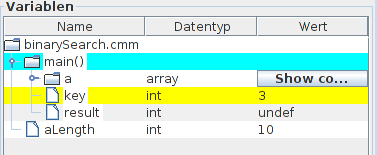
\includegraphics[width=1.0\textwidth]{./media/images/gui/var/tt-norender.png}
		\caption{TreeTable ohne Renderer für den JTree}\label{fig:deb-tt-render-no}
	\end{minipage}\hfill
	\begin{minipage}{0.48\textwidth}
		\centering
		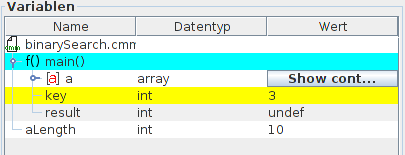
\includegraphics[width=1.0\textwidth]{./media/images/gui/var/tt-render.png}
		\caption{TreeTable mit Renderer für den JTree}\label{fig:deb-tt-render-no}
	\end{minipage}
\end{figure}

%    ---------------------------------------------------------------------
%        Spezielle Implementierung
%    ---------------------------------------------------------------------
\subsection{Implementierung für den Debugger}
Hier werden die Erweiterungen an der TreeTable beschrieben, die für die Anwendung im Debugger nötig waren. Für andere Anwendungsfälle kann ähnlich verfahren werden.

\subsubsection*{VarTreeTable.java}
VarTreeTable ist eine Wrapperklasse für TreeTable. Sie übernimmt alle wichtigen Funktionen zur Kommunikation mit dem Variablenbaum und bildet so eine Schicht zwischen dem Debugger und der TreeTable. Auf diese Weise wird der Code übersichtlicher und ist besser strukturiert.
TreeTableView hat folgende Methoden:
\begin{itemize}
\item \textbf{init} Initialisiert die TreeTable mit einem Standard-Datenmodell. Dieses besteht nur aus einem Hauptknoten (root), der den Namen der aktuellen Datei trägt; es werden keine Variablen angezeigt. Das Standard-Datenmodell wird immer dann angezeigt, wenn der Debugger nicht aktiv ist, also wenn der Benutzer den Sourcecode editiert.
\item \textbf{standby} Löscht das aktuelle Datenmodell und übergibt ein Standard-Datenmodell an die TreeTable, sodass wie zu Beginn nur der aktuelle Dateiname angezeigt wird. Diese Methode wird immer aufgerufen, wenn der Debugger beendet wird.
\item \textbf{update} Aktualisiert das Datenmodell der TreeTable im Debugmodus und zeigt die Variablen im Speicher des Interpreters an.
\item \textbf{highlightVariable} Mit dieser Methode wird die Addresse einer zuletzt geänderten Variable an die TreeTable übergeben. Diese Variable wird in der Tabelle markiert. Es ist möglich, diese Funktion mehrmals aufzurufen und so mehrere Variablen zu markieren. Wenn das Datenmodell mit \textbf{update} aktualisiert wird, verfallen alle Addressen.
\item \textbf{updateFontSize} Bei Aufruf dieser Methode wird die Schriftgröße der Tabelle geändert und die gesamte TreeTable neu gezeichnet. Diese Methode wird aufgerufen, wenn die Einstellungen der Benutzeroberfläche geändert wurden.
\end{itemize}

\subsubsection*{VarDataNode.java}
Die Klasse VarDataNode erweitert die abstrakte Klasse DataNode und kann deshalb für die Datenstruktur der TreeTable verwendet werden. Ein VarDataNode bildet einen Knoten im Baum bzw. eine Zeile in der TreeTable.

Folgende Daten werden in einem Knoten gespeichert:
\begin{lstlisting}[language=JAVA]
// Informationen, die in der Tabelle angezeigt werden
private final String name;
private Object type;
private Object value;

// Zusätzliche Informationen
private int address;
\end{lstlisting}
Die Felder für Datentyp und Wert haben den Typ Object, da sich in der Tabelle an der Stelle eines Wertes auch ein JButton befinden kann.
%TODO refer to JTableButtonRenderer.java

Zusätzlich werden die Adresse und die Deklarationszeile der Variable gespeichert. Die Adresse dient der eindeutigen Identifikation der Variable, zum Beispiel beim Traversieren durch den Variablenbaum. Dadurch können lokale Variablen auch bei mehrfachem Aufruf einer Funktion unterschieden werden.
%TODO add more information about Methods, ...

\subsubsection*{TreeStructImageRenderer.java}
Dieser Renderer wird anstelle des Standardrenderers \textbf{TreeRenderer} der TreeTable verwendet. Wie im TreeRenderer sind auch hier Methoden implementiert, um die Hintergrundfarben der Knoten des JTree zu entfernen. Außerdem ist eine weitere Methode implementiert, die den Knoten des Baumes je nach Datentyp ein anderes Icon gibt.

Zum Ändern des Icons eines Knoten muss im Renderer folgende Methode implementiert werden:
\begin{lstlisting}[language=JAVA]
public JComponent getTreeCellRendererComponent(JTree tree, Object value, boolean sel, boolean exp, boolean leaf, int row, boolean hasFocus) {

	ImageIcon icon = new ImageIcon("images/icon.png");

	setOpenIcon(icon);
	setClosedIcon(icon);
	setLeafIcon(icon);
	
	super.getTreeCellRendererComponent(tree, value, sel, exp, leaf, row, hasFocus);
		
	return this;
}
\end{lstlisting}

Für unterschiedliche Arten von Variablen werden unterschiedliche Bilder verwendet:
\def\arraystretch{1.4}
\begin{table}[h!]
\center
\begin{tabular}{|cl|}
\hline 
Bild & Art des Eintrages \\ 
\hline

\includegraphics[scale=1.0]{./media/images/gui/var/icons/cmm.png} & Hauptknoten: Die CMM-Datei selbst \\
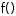
\includegraphics[scale=1.0]{./media/images/gui/var/icons/func.png} & Funktionen \\

\includegraphics[scale=1.0]{./media/images/gui/var/icons/struct.png} & Strukturen \\ 

\includegraphics[scale=1.0]{./media/images/gui/var/icons/array.png} & Arrays (nur der übergeordnete Knoten, nicht die Indizes) \\ 
- & Einfache Datentypen haben kein Bild\\
\hline 
\end{tabular}
\caption{Icons für unterschiedliche Strukturen und Einträge in der Variablentabelle}
\end{table}

